\pagebreak
\section*{11. What Is Bitcoin Mining?}
\addcontentsline{toc}{chapter}{What Is Bitcoin Mining?}
Bitcoin mining is the process by which new bitcoins are entered into circulation, but it is also a critical component of the maintenance and development of the blockchain ledger. It is performed using very sophisticated computers that solve extremely complex computational math problems.\vspace{.3cm}

Cryptocurrency mining is painstaking, costly, and only sporadically rewarding. Nonetheless, mining has a magnetic appeal for many investors interested in cryptocurrency because of the fact that miners are rewarded for their work with crypto tokens. This may be because entrepreneurial types see mining as pennies from heaven, like California gold prospectors in 1849. And if you are technologically inclined, why not do it?\vspace{.3cm}

However, before you invest the time and equipment, read this explainer to see whether mining is really for you. We will focus primarily on Bitcoin (throughout, we'll use "Bitcoin" when referring to the network or the cryptocurrency as a concept, and "bitcoin" when we're referring to a quantity of individual tokens).\vspace{.3cm}

\begin{figure}[h]
	\centering
	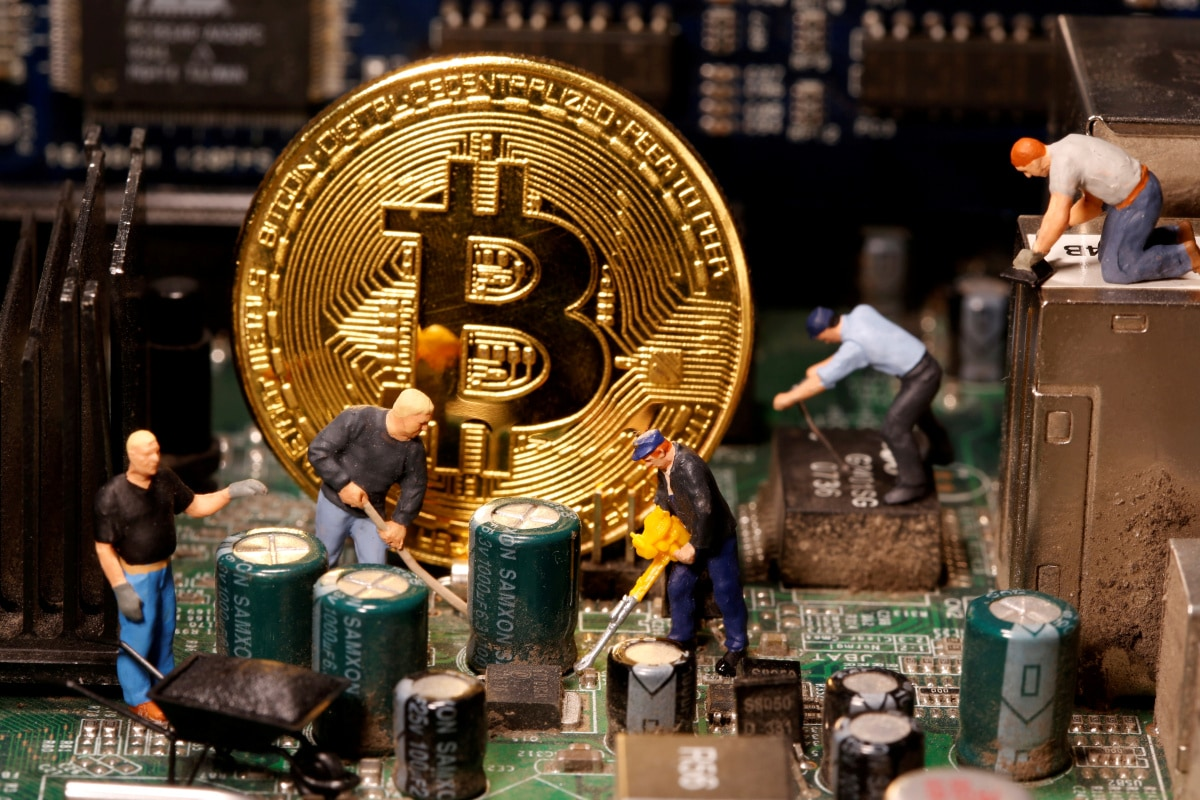
\includegraphics[width=0.7\linewidth]{bitcoin_colours_reuters_1611921415626}
	\captionsetup{labelformat=empty}
	\caption{Bitcoin Mining}
\end{figure}

\subsection*{11.1 How to Mine Bitcoins}

Miners are getting paid for their work as auditors. They are doing the work of verifying the legitimacy of Bitcoin transactions. This convention is meant to keep Bitcoin users honest and was conceived by Bitcoin's founder, Satoshi Nakamoto. By verifying transactions, miners are helping to prevent the "double-spending problem." \vspace{.3cm}

Double spending is a scenario in which a Bitcoin owner illicitly spends the same bitcoin twice. With physical currency, this isn't an issue: once you hand someone a \$20 bill to buy a bottle of vodka, you no longer have it, so there's no danger you could use that same \$20 bill to buy lotto tickets next door. While there is the possibility of counterfeit cash being made, it is not exactly the same as literally spending the same dollar twice. With digital currency, however, as the Investopedia dictionary explains, "there is a risk that the holder could make a copy of the digital token and send it to a merchant or another party while retaining the original."\vspace{.3cm}

Let's say you had one legitimate \$20 bill and one counterfeit of that same \$20. If you were to try to spend both the real bill and the fake one, someone that took the trouble of looking at both of the bills' serial numbers would see that they were the same number, and thus one of them had to be false. What a Bitcoin miner does is analogous to that—they check transactions to make sure that users have not illegitimately tried to spend the same bitcoin twice. This isn't a perfect analogy—we'll explain in more detail below.\vspace{.3cm}

Once miners have verified 1 MB (megabyte) worth of Bitcoin transactions, known as a "block," those miners are eligible to be rewarded with a quantity of bitcoins (more about the bitcoin reward below as well). The 1 MB limit was set by Satoshi Nakamoto, and is a matter of controversy, as some miners believe the block size should be increased to accommodate more data, which would effectively mean that the bitcoin network could process and verify transactions more quickly.\vspace{.3cm}

Note that verifying 1 MB worth of transactions makes a coin miner eligible to earn bitcoin—not everyone who verifies transactions will get paid out.\vspace{.3cm}

1MB of transactions can theoretically be as small as one transaction (though this is not at all common) or several thousand. It depends on how much data the transactions take up.\vspace{.3cm}